\section{Apéndice I: Clasificación de la bibliografía recopilada}
\label{tablabiblio}
A continuación se muestra una tabla con la clasificación de los documentos recopilados durante la etapa de investigación en este proyecto.

Los mismos están clasificados según las etapas que componen el sistema y tienen un código de color de acuerdo a la relevancia que tienen para el proyecto:
\begin{itemize}
	\item Verde: el documento contiene información de valor para el proyecto, por lo que debe tenerse en cuenta.
	\item Amarillo: la información contenida en el documento, si bien está relacionada con la categoría en la cual está ubicada, no contiene la metodología elegida para la implementación, o no aporta información de valor. 
\end{itemize}

Además, se agregan comentarios sobre el contenido de los documentos, el año en que fueron publicados, cantidad de citas en otras publicaciones, y ventajas y desventajas de la metodología aplicada.

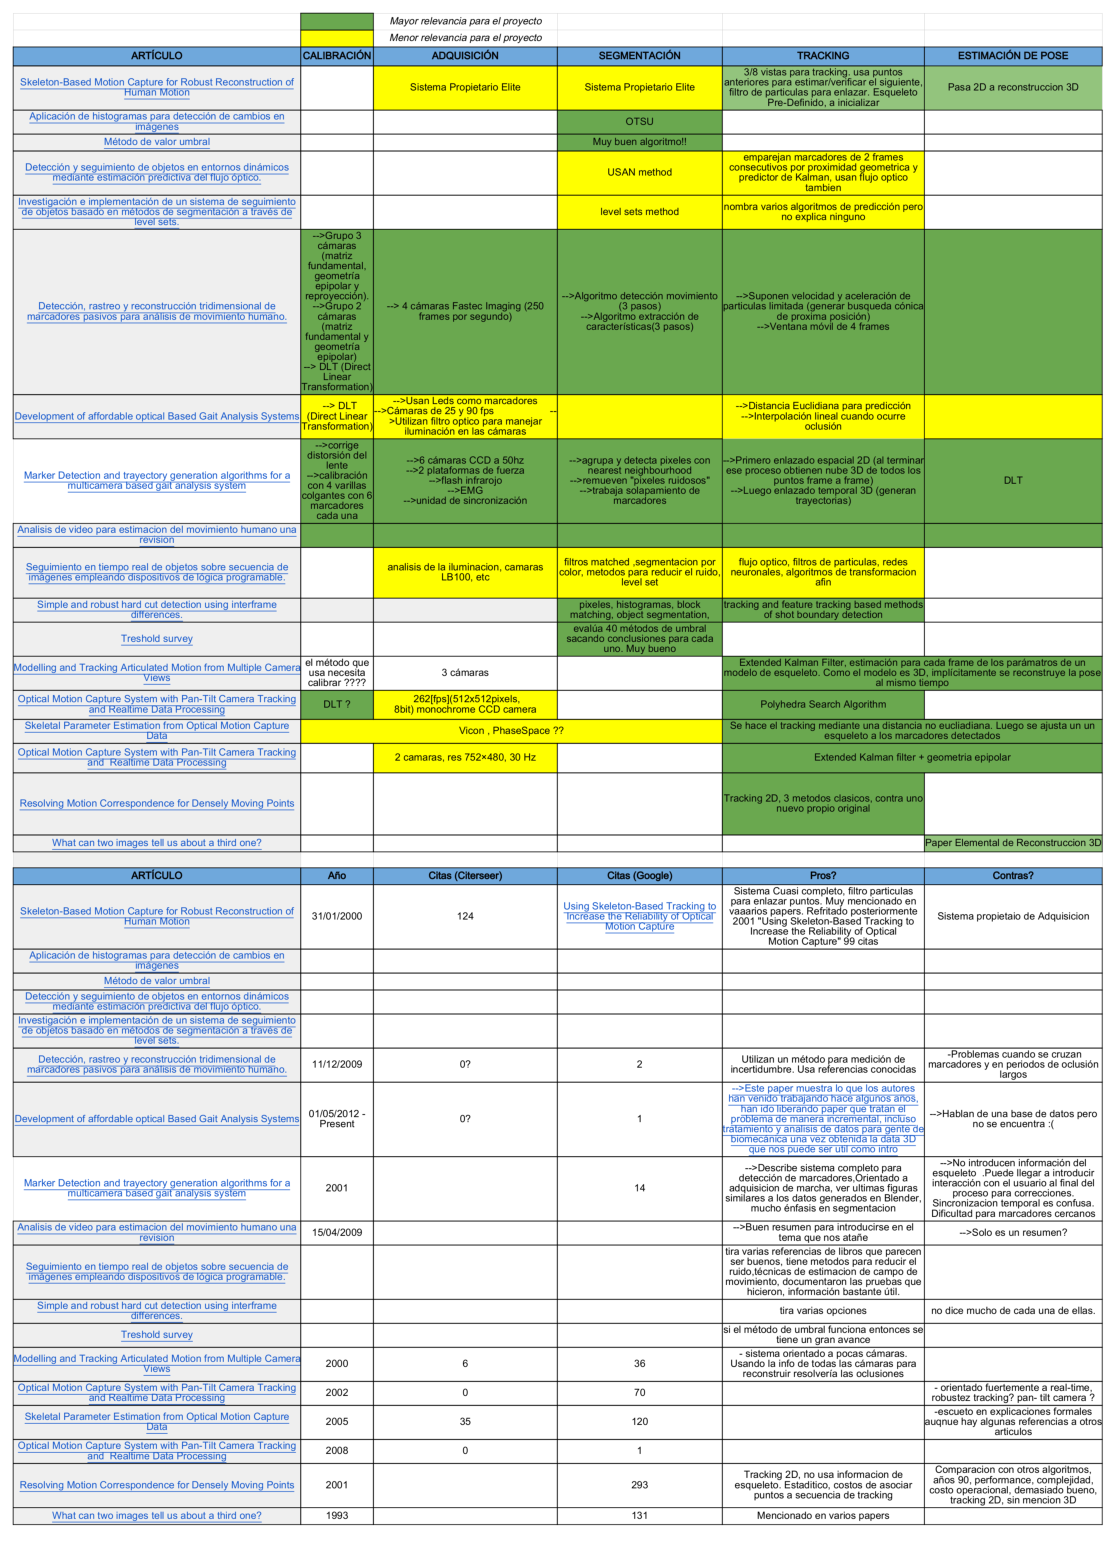
\includepdf[pages={1}]{Resumen_bibliografia.pdf}
